\chapter{Higgs Phenomology}
\label{sec:pheno}

Dasu -
The pheno chapter need not start from the Dirac equation and build up. It should have crisp intro to Higgs phenomenology starting from that portion of the Lagrangian. You don’t need all the myriad details of SM like the quark mixing matrices, etc.


In this chapter I provide an increasingly mathematical description of the standard model
of physics, specifically in reference to the Higgs boson. I provide a basic overview of some 
properties of the Higgs boson including how it is created in a hadron collider, an overview
of the possible decay paths for a Higgs boson, and a discussion of the Higgs boson
couplings, or interactions, with different fundamental particles. A description of the
Higgs boson requires covering the process of electroweak symmetry breaking (EWSB) which
provides the mathematical descripition of the process defining the Higgs boson and the
Higgs field.

\section{Standard Model Symmetries}
Many people are attracted to physics because of the beauty they see in the patterns of nature.
PW Anderson, a physics Nobel laureate, stated, ``it is only slightly overstating the case 
to say that physics is the study of symmetry''~\cite{pw_anderson:1972}.
One way of expressing many types of patterns mathematically is with symmetries, properties which 
remain invariant under certain transformations. The SM is defined by a group of symmetries
representing certain conserved properties. Specifically, the SM is represented by  the
symmetries of the unitary product group SU(3)$_{\text{C}} \times$ SU(2)$_{\text{L}} \times$ U(1)$_{\text{Y}}$.
These three terms all reflect symmetries and conserved quantities discussed below.

Electric charge ($Q$), the third component of weak isospin ($T_{3}$), and hypercharge ($Y$) act together to define a conserved 
quantity in the SM, $Q = T_{3} + \frac{Y}{2}$. This is represented by the
hypercharge U(1)$_{\text{Y}}$ symmetry group.

The two SU($n$) groups are special unitary groups which represent rotations.
In the SM, the SU(2) group provides a description of particle spin.
The ``L'' subscript for the SU(2)$_{\text{L}}$ group indicates that that it only couples to
and describest left handed fermions.
The SU(3)$_{\text{C}}$ group describes the local symmetry of color charge conservation.


\section{Electroweak Symmetry Breaking}
In the SM, the electromagnetic force and weak force are described together by
the electroweak Lagrangian~\cite{Glashow:1961tr,SM1,SM3}.
Prior to the introduction of Electroweak Symmetry Breaking (EWSB),
the electroweak Lagrangian describes massless $\PW$ and $\PZ$ bosons.
EWSB rescues what would be a collasal disagreement between theoretical prediction
and experimental results. The introduction of EWSB to the theory preserves the structure of
the electroweak interactions and succeedes in endowing the $\PW$ and $\PZ$ bosons
with mass.

The electroweak Lagrangian defines a gauge field theory which is 
invariant under the SU(2)$_{\text{L}} \, \times \, $U(1)$_{\text{Y}}$ symmetry group. 





The EWSB mechanism posits a self-interacting complex doublet scalar field, whose CP-even neutral component acquires a vacuum expectation value (VEV) v ≈ 246GeV, which sets the scale of electroweak symmetry breaking. Three massless Goldstone bosons are generated and are absorbed to give masses to the W and Z gauge bosons. The remaining component of the complex doublet becomes the Higgs boson – a new fundamental scalar particle. The masses of all fermions are also a consequence of EWSB since the Higgs doublet is postulated to couple to the fermions through Yukawa interactions.


The Higgs boson must have couplings to W/Z gauge bosons and fermions precisely as those in the SM to maintain the consistency of the theory at high energies, hence, formally there is no need for new physics at the EW scale.



the spontaneous breaking of the SM gauge symmetry SU(3)C × SU(2)L × U(1)Y into SU(3)C × U(1)em

electroweak symmetry breaking is achieved via the Brout--Englert--Higgs
mechanism~\cite{Englert:1964et,Higgs:1964ia,Higgs:1964pj,Guralnik:1964eu,Higgs:1966ev,Kibble:1967sv},
leading, in its minimal version, to the prediction of the existence of one physical neutral scalar particle,
commonly known as the Higgs boson ($\PH$).


\section{Higgs Yukawa Couplings}
To establish the mass generation mechanism for fermions,
 it is necessary to probe the direct coupling of
the Higgs boson to such particles.
The most promising decay channel is $\Pgt^+\Pgt^-$,
because of the large event rate expected in the SM compared to the $\Pgm^+\Pgm^-$ decay channel ($\mathcal{B}(\PH\to\Pgt^+\Pgt^-)=6.3$\% for a mass of 125.09\GeV), and of the smaller contribution from background events
with respect to the $\bbbar$ decay channel.

\section{Higgs Production}

Feynman diagrams for the leading Higgs boson production processes
are shown in Figure~\ref{fig:higgs_feyn}.

\begin{figure*}[htbp]
\centering
     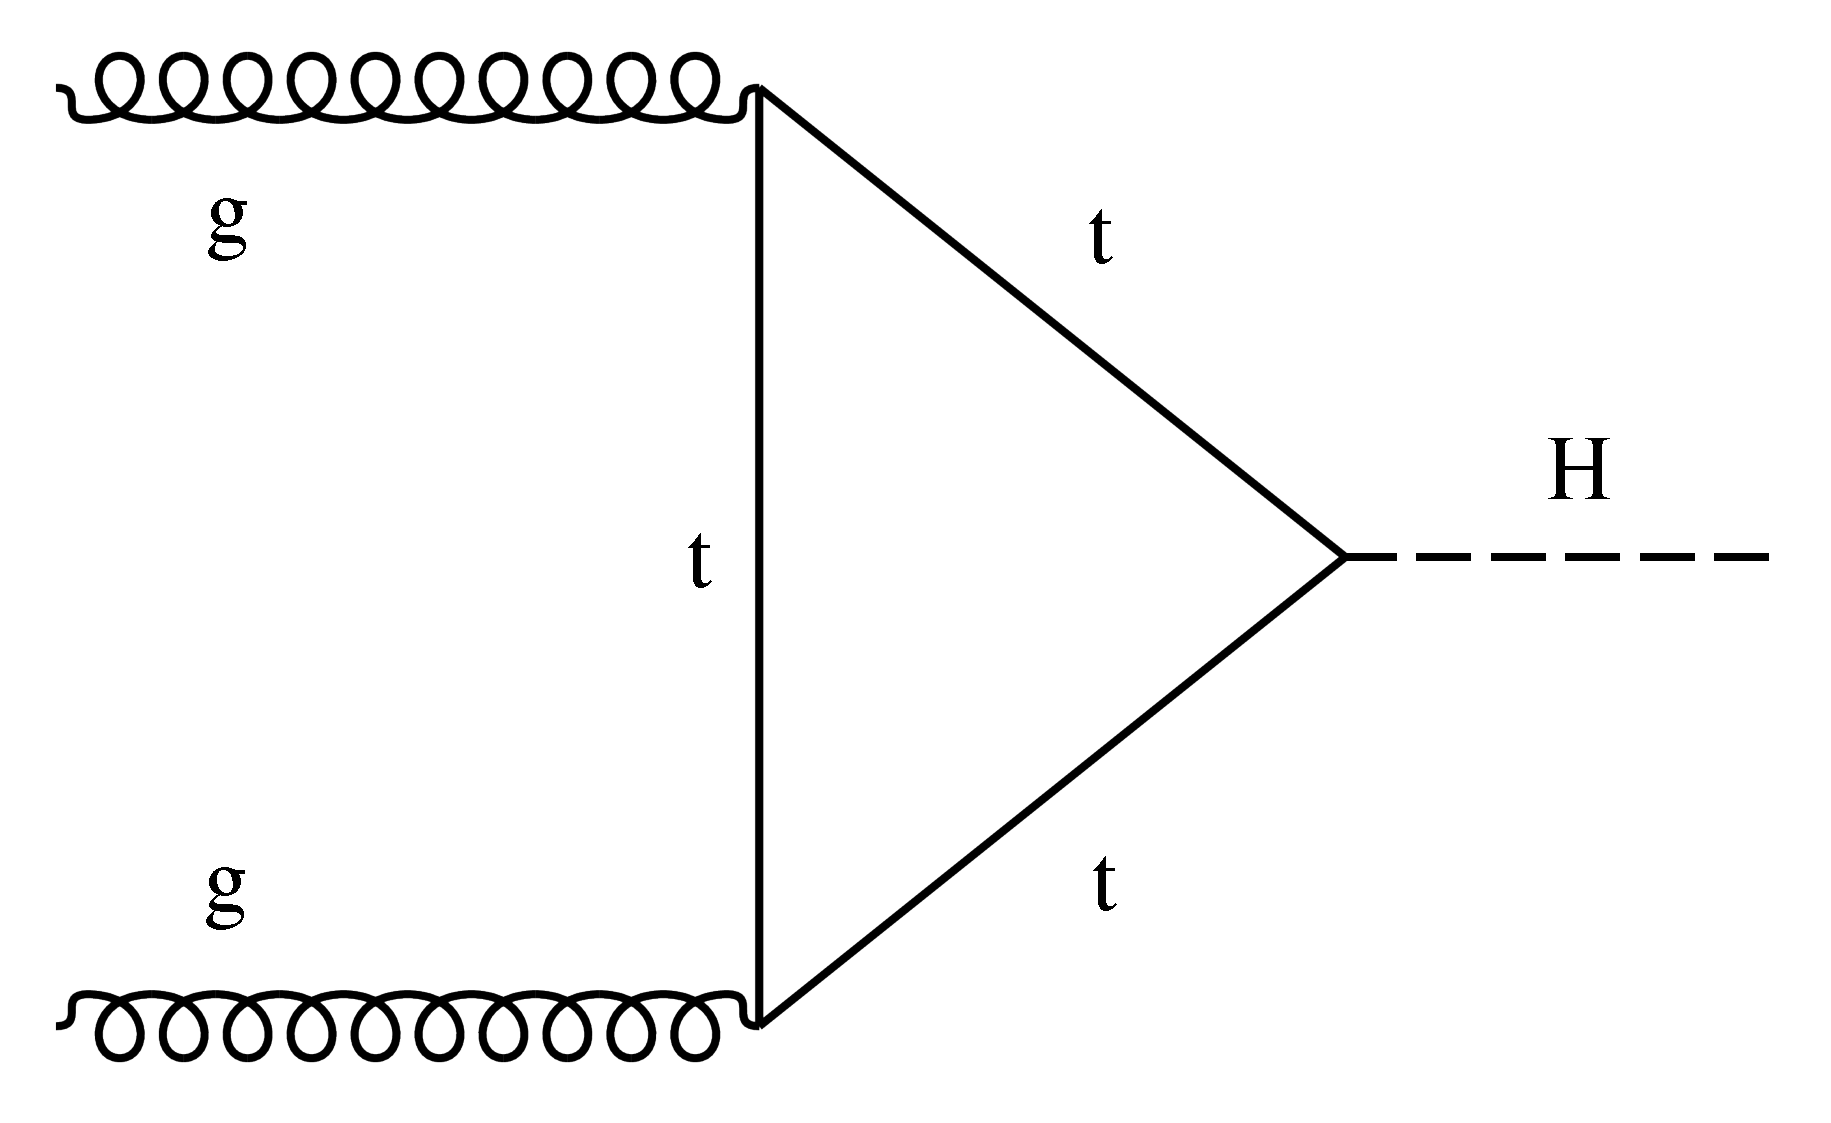
\includegraphics[width=0.35\textwidth]{phenomology_of_processes/plots/feyn_ggH.pdf}
     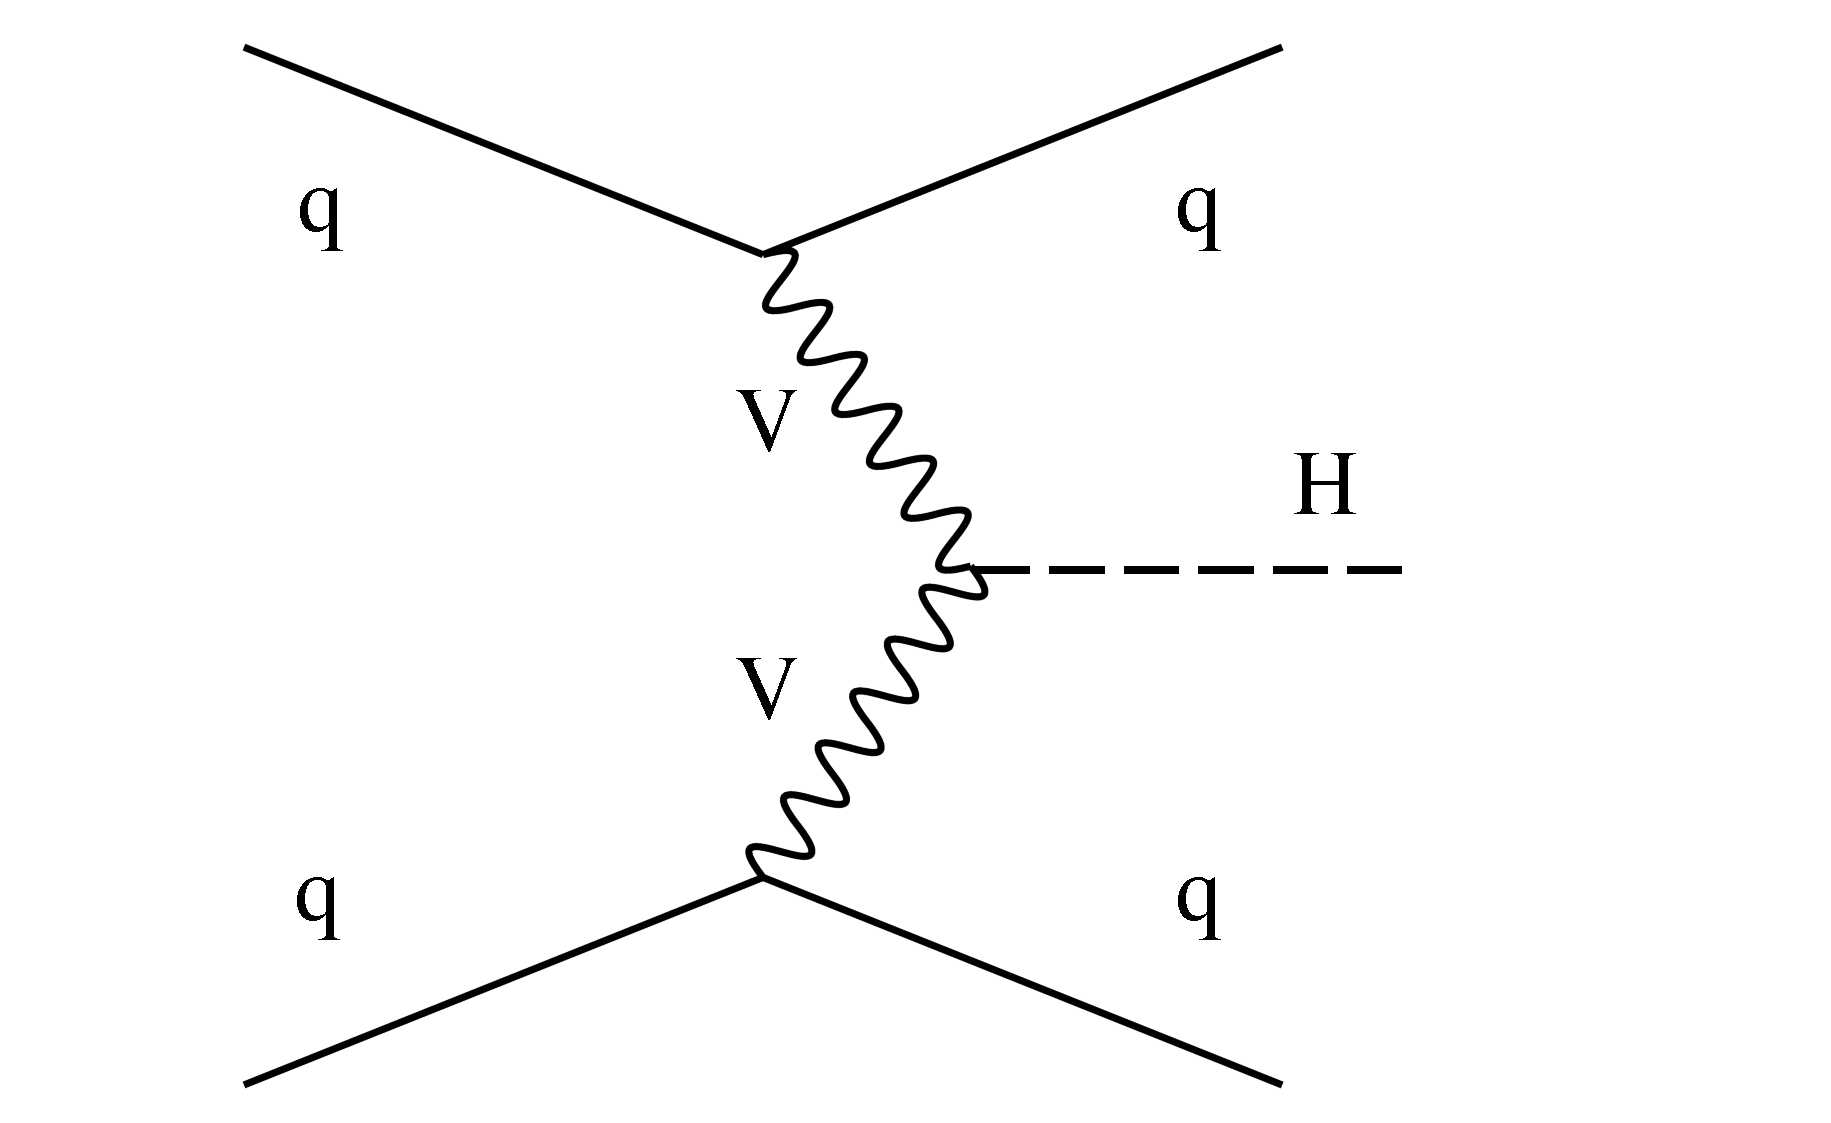
\includegraphics[width=0.35\textwidth]{phenomology_of_processes/plots/feyn_qqH.pdf}
     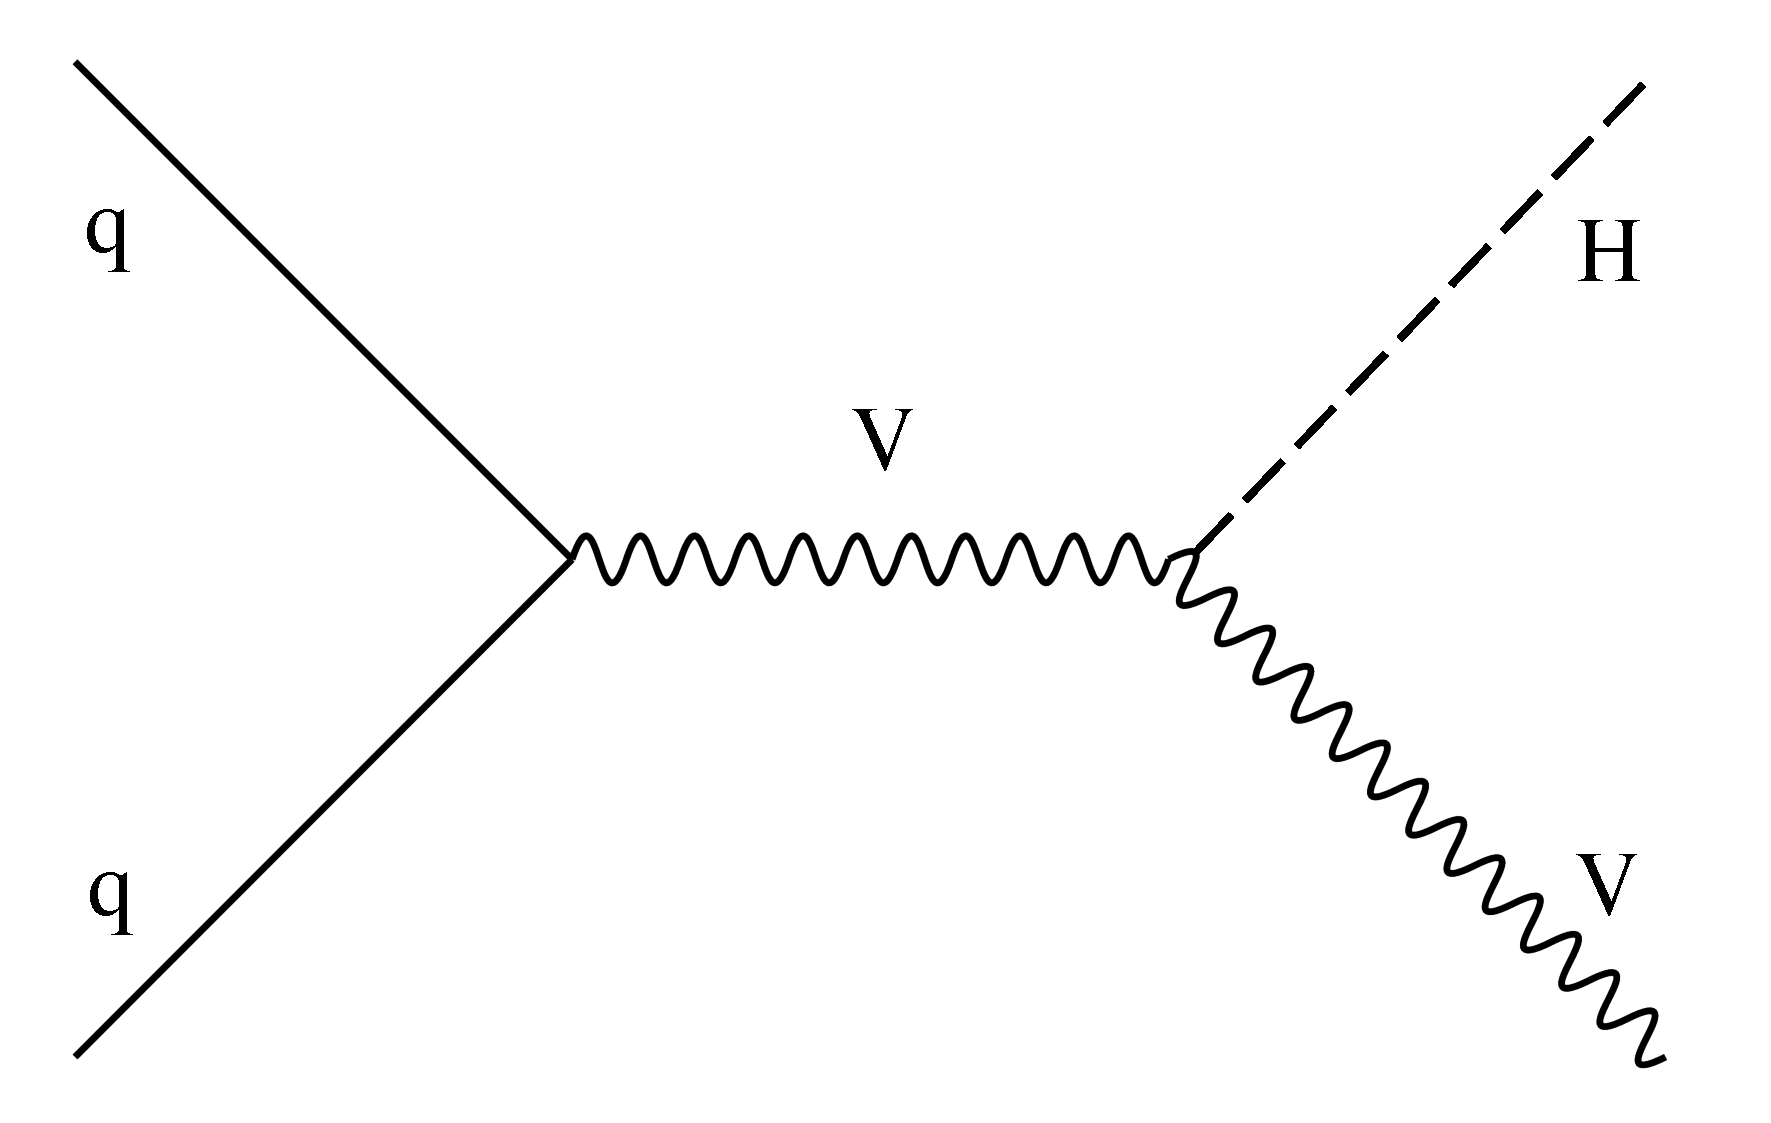
\includegraphics[width=0.35\textwidth]{phenomology_of_processes/plots/feyn_VH.pdf}
     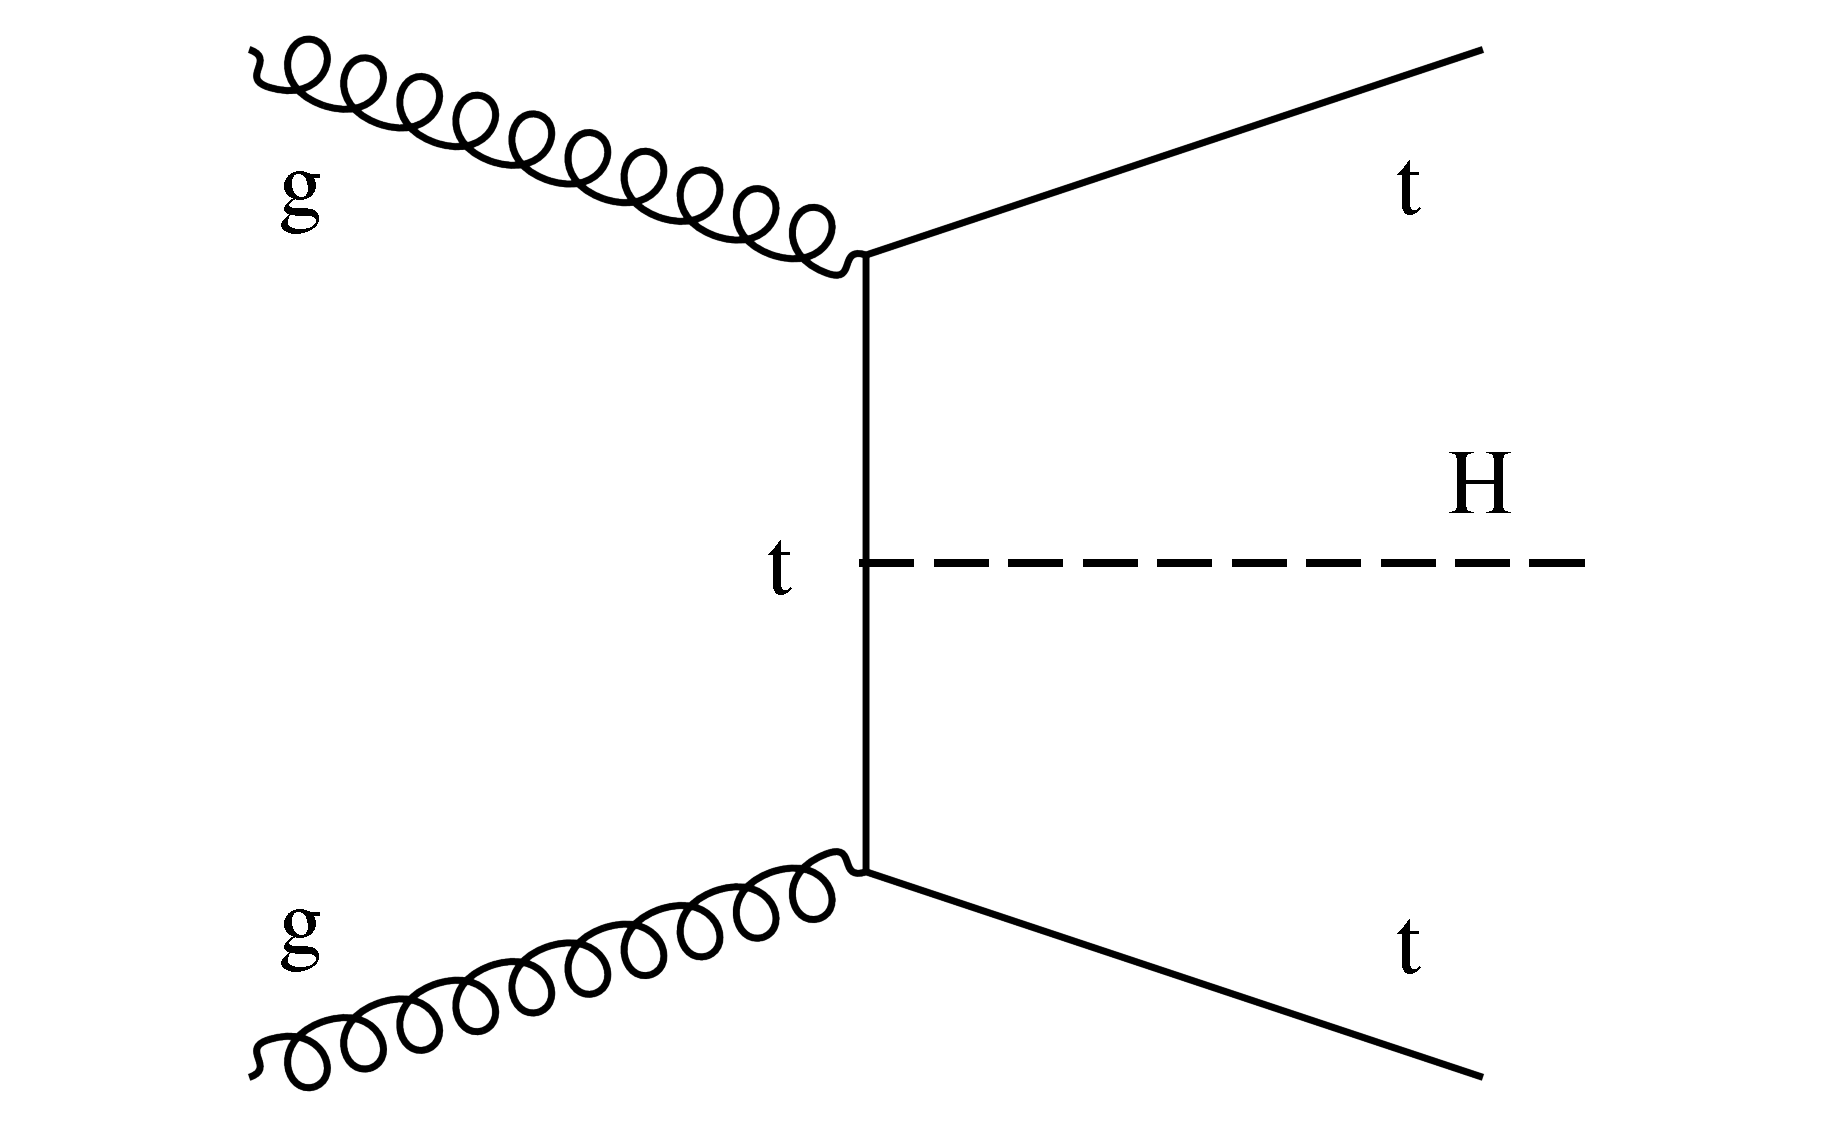
\includegraphics[width=0.35\textwidth]{phenomology_of_processes/plots/feyn_ttH.pdf}
     \caption{
Feynman diagrams representing the leading Higgs boson production processes.
Progressing in order of largest to smallest of these production cross sections:
(top left) gluon fusion, (top right) vector boson fusion, (bottom left)
associated production covering both the $\PW\PH$ and $\PZ\PH$ processes,
and (bottom right) top-quark associated production.
     }
     \label{fig:higgs_feyn}
\end{figure*}

The cross sections for the leading Higgs boson production processes
are shown in Figure~\ref{fig:higgs_production}. The values for the leading
process are approximately: $ggH \approx 49\pb$, VBF$ \approx 3.8\pb$, $\PW\PH \approx 1.4\pb$,
and $\PZ\PH \approx 0.88\pb$~\cite{deFlorian:2016spz}. The $\ttbar\PH$ process,
which is found to be relatively insignificant in the following analyses, has a cross
section approximatly half the size of the next smallest one, $\PZ\PH$, where
$\ttbar\PH \approx 0.51\pb$.


\begin{figure*}[htbp]
\centering
     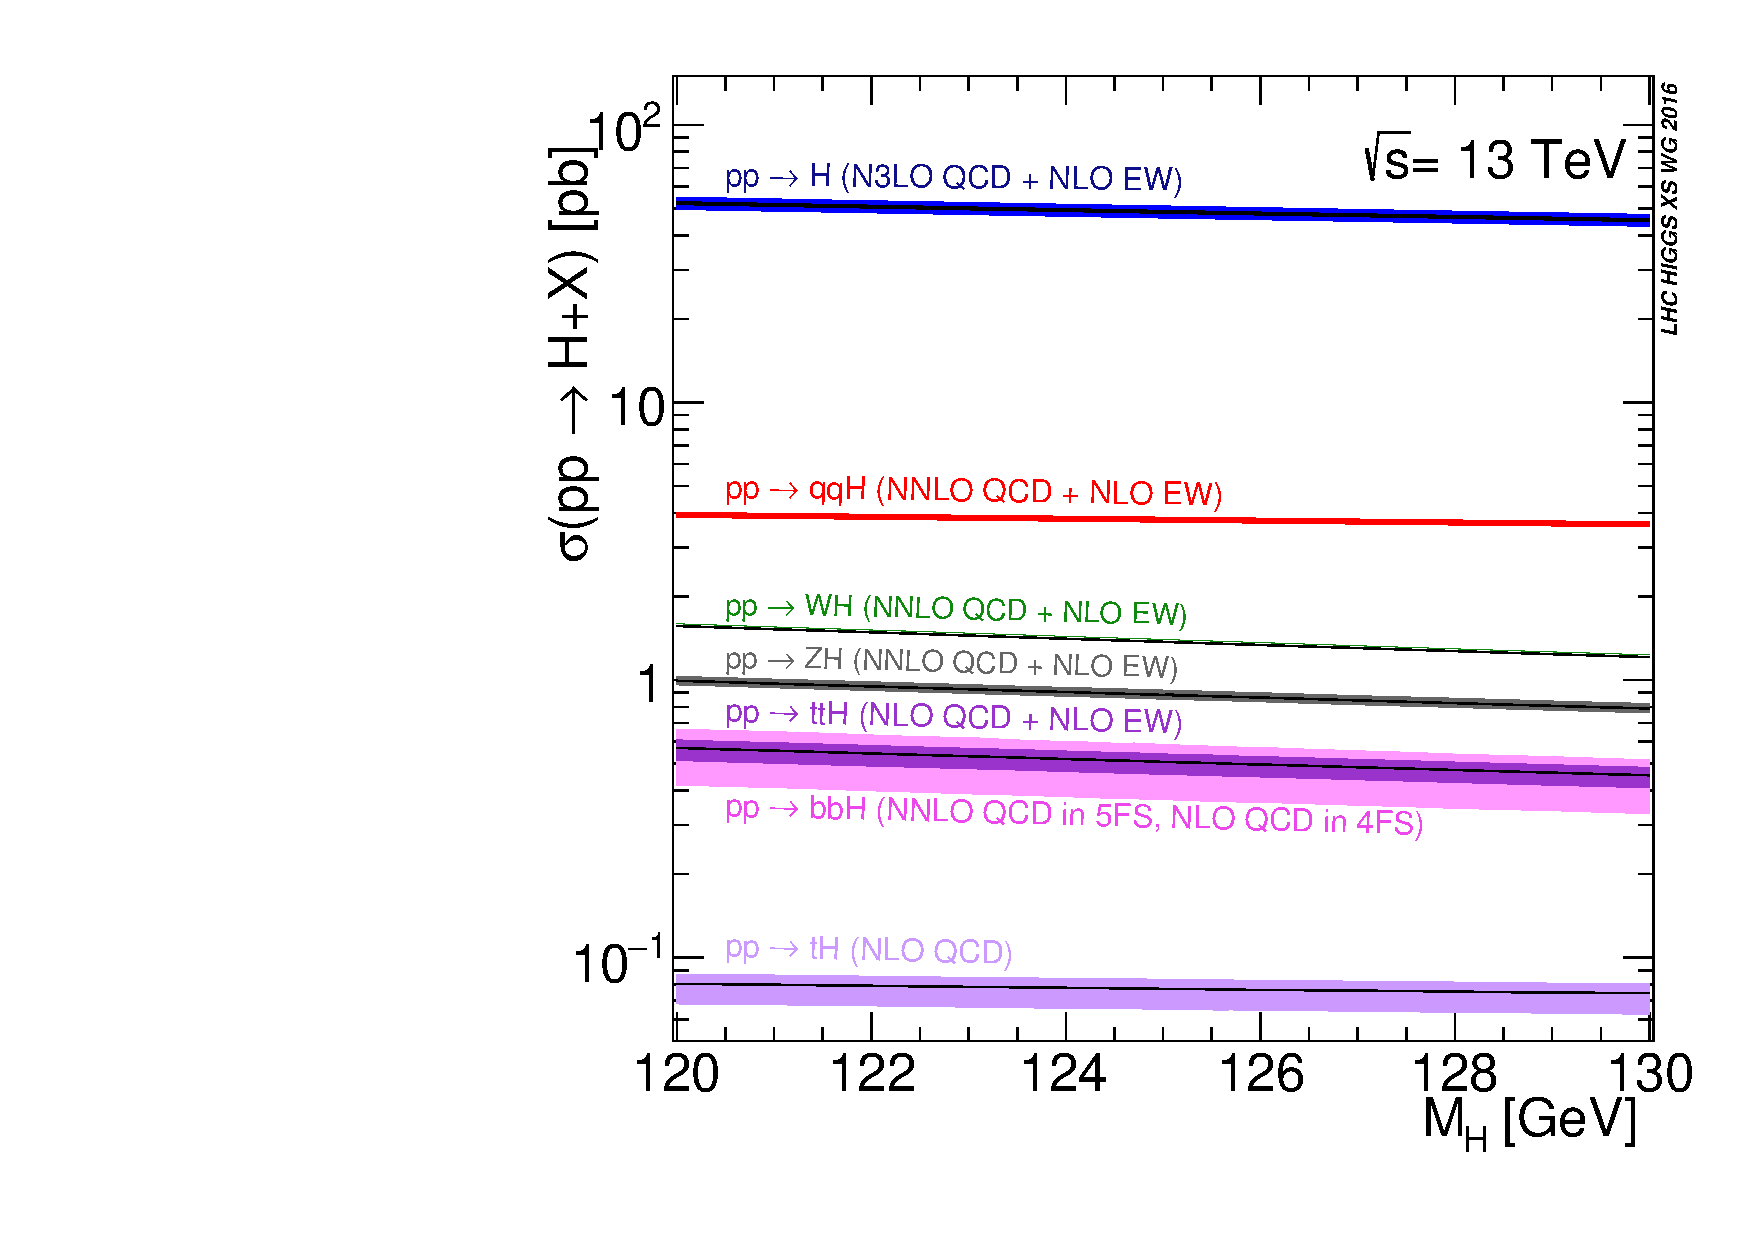
\includegraphics[width=0.65\textwidth]{phenomology_of_processes/plots/plot_13tev_H_sqrt.pdf}
     \caption{
The theorized Higgs boson production cross sections and their uncertainties,
as a function of the Higgs boson mass, are shown. The gluon fusion process ($ggH$)
is denoted as pp $\to$ H in the figure.
The CMS and ATLAS experiments have determined $\mH = 125.09\GeV$~\cite{Aad:2015zhl}.
     }
     \label{fig:higgs_production}
\end{figure*}


\subsection{Gluon Fusion}
$ggH$ - mediated by the exchange of a virtual, heavy top quark, Contributions from lighter quarks propagating in the loop are suppressed proportional to $m^{2}_{q}$.
To a very good approximation, the leading top-quark contribution can be evaluated in the limit $m_{t} \to \inf$ [24,25].

\subsection{Vector Boson Fusion}
Higgs production via VBF, qq → qqH, proceeds by the scattering of two (anti-)quarks, mediated by t- or u-channel exchange of a W or Z boson, with the Higgs boson radiated off the weak-boson propagator. The scattered quarks give rise to two hard jets in the forward and backward regions of the detector. Because of the color-singlet nature of the weak-gauge boson exchange, gluon radiation from the central-rapidity regions is strongly suppressed. These characteristic features of VBF processes can be exploited to distinguish them from overwhelming QCD backgrounds, including gluon-fusion induced Higgs + 2 jet production, and from s-channel WH or ZH production with a hadronically decaying weak gauge boson. After the application of specific selection cuts, the VBF channel provides a particularly clean environment, not only for Higgs searches but also for the determination of Higgs boson couplings at the LHC [74].

\subsection{Associated Production}

\section{Higgs Decays}

After a Higgs boson is produced, it will decay extremly rapidly. The theorized lifetime of a Higgs
boson particle is $1.6 \times 10^{-22}$ s~\cite{Dittmaier:2012vm} meaning that, when created
inside of the CMS detector, a Higgs boson will always decay
within the CMS detector . There are multiple possible decay
paths each with their own probability or branching ratio with the largest branching ratio
processes shown in Figure~\ref{fig:higgs_decay}. The $\htt$ process has a branching
ratio of approximately 6.3\% for $\mH = 125\GeV$.


\begin{figure*}[htbp]
\centering
     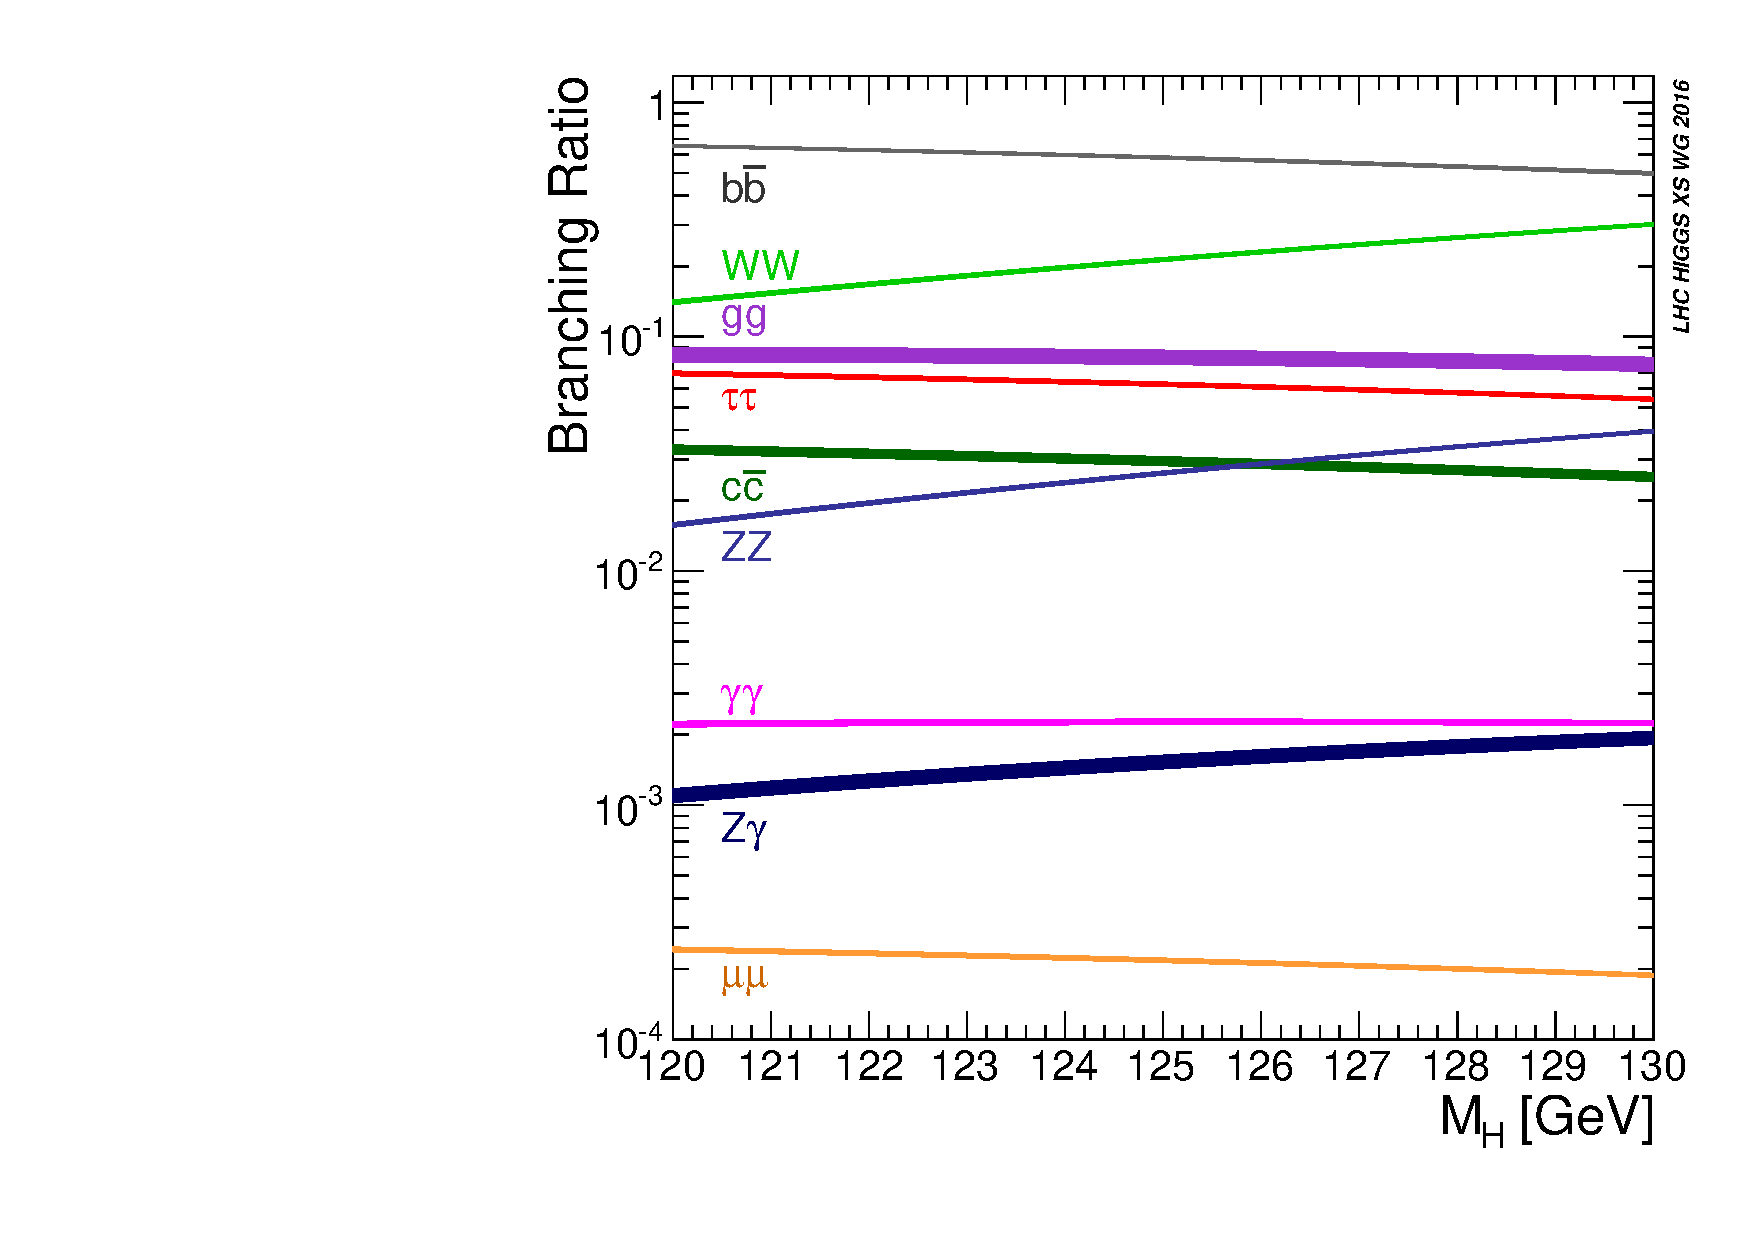
\includegraphics[width=0.65\textwidth]{phenomology_of_processes/plots/SMHiggsBR_YR4-square.pdf}
     \caption{
The different theorized Higgs boson decay process are shown as a 
as a function of the Higgs boson mass.
The CMS and ATLAS experiments have determined $\mH = 125.09\GeV$~\cite{Aad:2015zhl}.
     }
     \label{fig:higgs_decay}
\end{figure*}


\subsection{Higgs to $\tau\tau$ Decay Process}

Estimated as 6.3\% with a relative theoretical uncertainty of $\pm5.7\%$~\cite{deFlorian:2016spz}.




The various production cross sections and branching fractions for the SM Higgs 
boson production, and their corresponding uncertainties are taken from 
References.~\cite{deFlorian:2016spz,Denner:2011mq,Ball:2011mu} and references therein.




%\subsection{QCD and Proton Structure}









